\documentclass[journal]{IEEEtran}

\usepackage[utf8]{inputenc}
\usepackage[T1]{fontenc}
\usepackage{hyperref}
\usepackage{url}
\usepackage{booktabs}
\usepackage{amsfonts}
\usepackage{amsmath}
\usepackage{amssymb}
\usepackage{mathtools}
\usepackage{amsthm}
\newtheorem{proposition}{Proposition}
\usepackage{graphicx}
\usepackage{xcolor}
\usepackage{microtype}
\usepackage{tabularx}
\usepackage{array}
\usepackage[backend=biber,style=ieee,sorting=none,maxbibnames=3,minbibnames=3]{biblatex}
\addbibresource{ref.bib}
\hypersetup{colorlinks=true,linkcolor=blue!50!black,citecolor=blue!50!black,urlcolor=blue!50!black}
\graphicspath{{figs/}}
\setlength{\belowcaptionskip}{0pt}

\newcommand{\eg}{\textit{e.g.,}\ }
\newcommand{\ie}{\textit{i.e.,}\ }
\newcommand{\etal}{\textit{et al.}}
\newcommand{\suppl}[1]{Supplement~#1}

\title{AutoResearch-Ledger: Transactional Revision Integrity for Executable Research Agents}

\author{
    Rajesh~Kumar, %
    \thanks{Rajesh Kumar is with the International Research Center for Complexity Sciences, Hangzhou International Innovation Institute, Beihang University, Hangzhou 311115, China (e-mail: rajakumarlohano@gmail.com).}%
    Waqar~Ali, %
    \thanks{Waqar Ali is with the Department of Computer Science, College of Science, Mathematics and Technology, Wenzhou-Kean University, Wenzhou 325060, China (e-mail: waqar.uestc@yahoo.com).}%
    Junaid~Ahmed, %
    \thanks{Junaid Ahmed is with Computer Systems Engineering Department, Sukkur IBA University, Sindh, Pakistan (e-mail: j.bhatti@iba-suk.edu.pk).}%
    Abdullah~Aman~Khan, %
    \thanks{Abdullah Aman Khan is with the International Research Center for Complexity Sciences, Hangzhou International Innovation Institute, Beihang University, Hangzhou 311115, China (e-mail: rajakumarlohano@gmail.com).}%
    Shaoning~Zeng %
    \thanks{Shaoning Zeng is with Yangtze Delta Region Institute (Huzhou), University of Electronic Science and Technology of China, Huzhou 313001, China (e-mail: zeng@csj.uestc.edu.cn).}%
}

\begin{document}
\maketitle

\begin{abstract}
Long-horizon research agents and executable paper agents can preserve outputs and draft manuscripts, yet a later code, data or evidence correction can leave stale downstream claims. We present AutoResearch-Ledger (TRL), a transactional research-state layer over executable provenance. \emph{Research state} denotes recorded commitments and declared dependencies, not truth. Claims use \emph{support sets}---jointly sufficient evidence sets plus necessary premises, non-epistemic dependencies and lineage---so conjunction and alternatives are representable where flat singleton support edges are not. Typed state machines separate provenance verification from scientific validity, while revisions propagate on a private copy before atomic commit or rollback. On synthetic conformance fixtures, full TRL matches an independently written oracle in 815/815 non-empty revision events. We additionally replayed 13 genuine historical scientific-software revisions across nine repositories; all 13 reproduced the documented semantic change. Executed as immutable old/new runs through a deterministic paper-agent proxy, all 13 completed the lifecycle \texttt{supported}$\rightarrow$\texttt{hypothesis}$\rightarrow$\texttt{supported}, and manuscript audit flagged explicit use of superseded evidence until replacement evidence was cited. Local transaction fault injection passed 6/6 checks, including exact restoration at all 11 tested entity-write failure positions. In an authored 10-event structural pilot, support-set provenance and full TRL achieved 10/10 exact impact identification, flat binary edges 6/10, and reachability/full rebuild 4/10. The integrated validation build passed 206/206 tests. We do not report an old/new Paper2Agent MCP replay or independent human annotation; these results establish implementation-level revision integrity under developer-authored bindings, not end-to-end scientific validity of real paper agents.
\end{abstract}

\begin{IEEEkeywords}
Research agents, provenance, transactional state, dependency propagation, truth maintenance, machine-checkable traceability.
\end{IEEEkeywords}

\section{Introduction}
\label{sec:intro}
\IEEEPARstart{R}{esearch} agents now search literature, formulate hypotheses, run code and draft manuscripts \cite{lu2026aiscientist,yamada2025aiscientistv2,schmidgall2025agentlab}. Paper2Agent extends this direction by converting papers, code, data and workflows into validated MCP-based executable agents that can reproduce analyses and answer new scientific queries \cite{miao2026paper2agent}. Recent work has also shifted attention from generation to \emph{verifiability}: ScientistOne maintains chains of evidence, EviGraph makes a typed evidence graph the agent's operational state, ARIS audits manuscript statements against a claim ledger, and claim-level provenance has been argued to be an evaluation target in its own right \cite{meng2026scientistone,ren2026evigraph,yang2026aris,rasheed2026auditability}. Agentification makes a remaining systems question more acute: after an upstream code, data, result or evidence correction, which previously generated outputs, claims, decisions and manuscript statements are still admissible? A corrected run can change one artifact while downstream state remains unchanged, even when both old and new software execute successfully: a \emph{stale dependency}.

We study this as a problem of \emph{revision semantics} over a typed, versioned research state (Fig.~\ref{fig:framework}). The Transactional Research Ledger (TRL) applies each change to a private copy, propagates it through the registered dependency graph, checks global invariants, and either commits a content-addressed snapshot or rolls back. Two design decisions carry most of the weight. First, a claim's dependence on evidence is not a set of independent edges: a claim that needs an experiment \emph{and} a robustness check survives the loss of one only if a different sufficient set remains. TRL therefore represents claims by \emph{support sets}. Second, the label ``verified'' is separated into what deterministic code can check (artifact, execution, result) and what it cannot (scientific validity), so that TRL never certifies more than it can inspect.

\begin{figure*}[t]
\centering
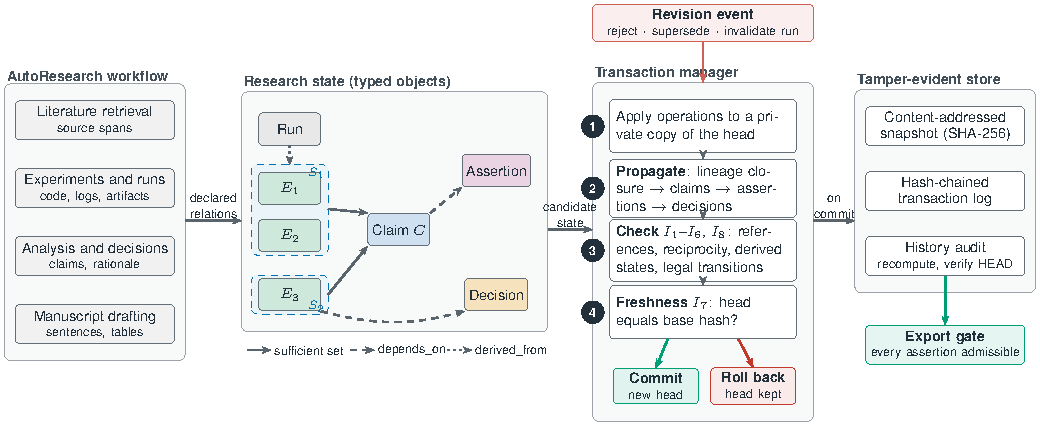
\includegraphics[width=\textwidth]{fig_framework.pdf}
\caption{TRL architecture. Pipeline stages register typed relations among runs, evidence, claims, decisions and manuscript assertions. A revision event enters the transaction manager, which applies it to a private copy, propagates it through the lineage closure, checks invariants $I_1$--$I_8$, and either commits a content-addressed, hash-chained snapshot or rolls back. The export gate admits a manuscript only if every assertion is admissible.}
\label{fig:framework}
\end{figure*}

We do not claim novelty for evidence graphs, provenance, truth maintenance or transactional agent state, nor for support sets themselves, which are the monotone fragment of ATMS labels and Boolean provenance (Section~\ref{sec:related}). As far as their published descriptions state, existing research agents provide evidence tracking, repair or audit; what we specify is \emph{atomic revision semantics} that propagate an invalidation through a typed research state with conjunctive and alternative dependencies. The contribution is this research-specific composition and its measurement, not a new formalism, and TRL is an execution engine for externally supplied dependency declarations, not a solution to acquiring them. The contributions are:
\begin{itemize}
    \item \textbf{Support-set dependency semantics} with necessary premises, non-epistemic dependencies and evidence lineage, strictly more expressive than flat singleton support-edge semantics (Section~\ref{sec:support}).
    \item \textbf{Typed state machines and provenance-verified evidence} with explicit tiers and an explicit exclusion of scientific validity (Section~\ref{sec:states}).
    \item \textbf{Atomic, tamper-evident revision} through invariants $I_1$--$I_8$, with a propagation soundness result scoped to the registered graph (Section~\ref{sec:txn}).
    \item \textbf{Dependency registration as a measured quantity}: precision, recall and support-set coverage, with flattened and spurious edges distinguished from missing ones (Sections~\ref{sec:registration}, \ref{sec:reg_results}).
    \item \textbf{A bridge validation on genuine revisions}: 13 historical semantic changes from nine repositories are replayed as old/new immutable runs through the implemented ledger, including claim invalidation, manuscript provenance audit and recovery (Section~\ref{sec:hist_replay_main}).
    \item \textbf{An instrument for confirmatory external validation}: a preregistered old/new executable-paper-agent protocol, blind annotation, an independent oracle, matched logical baselines and repository-clustered uncertainty (Section~\ref{sec:design}).
\end{itemize}
Our questions are: \textbf{RQ1} does TRL preserve invariants and prevent stale claims \emph{given a registered graph}; \textbf{RQ2} which mechanisms are necessary, including support sets and lineage; \textbf{RQ3} is its state machine-checkable (deterministic validation, rollback, tamper-evident history) and practical up to $10^5$ triples; \textbf{RQ4} how sensitive is protection to registration quality; \textbf{RQ5} can genuine historical semantic revisions be carried through immutable runs, evidence supersession, claim invalidation, manuscript audit and recovery in the implemented ledger; and \textbf{RQ6} how well do independently generated real paper agents register dependencies and preserve scientific state under genuine revisions. RQ1--RQ4 are answered with mechanism experiments, RQ5 with a developer-run tracked-proxy bridge study, and RQ6 and all human-audit claims remain open. Extended tables, protocols and proofs are in the Supplement (\suppl{S1}--S10).

\section{Related Work}
\label{sec:related}
\paragraph{Research agents and evidence assurance}
The AI Scientist, its tree-search successor and Agent Laboratory connect ideation, experimentation and writing \cite{lu2026aiscientist,yamada2025aiscientistv2,schmidgall2025agentlab}. Paper2Agent converts a paper and its public computational assets into tested MCP tools and reports robustness to several execution-level repository defects \cite{miao2026paper2agent}. That addresses whether a paper agent can be made executable and kept available; our target is complementary: whether \emph{persisted downstream research state} remains admissible after a scientifically consequential upstream revision, including a revision for which both versions still execute. ScientistOne requires generated claims to stay traceable to evidence across the lifecycle; EviGraph repairs downstream subgraphs when a weak dependency is found; ARIS audits manuscript statements against a claim ledger and raw evidence \cite{meng2026scientistone,ren2026evigraph,yang2026aris}. Auditability itself has been proposed as an evaluation dimension \cite{rasheed2026auditability,martinboyle2026papertrail}; we do not evaluate it, as we ran no human study. None of these was run head-to-head with TRL; \suppl{S8} tabulates their reported mechanisms.

\paragraph{Truth maintenance, belief revision and argumentation}
Justification-based truth maintenance labels nodes IN or OUT from justifications and revises dependents when an assumption is withdrawn \cite{doyle1979tms}; assumption-based maintenance instead labels each node with the minimal sets of assumptions (environments) under which it holds and answers queries in any context \cite{dekleer1986atms}. TRL's claim liveness is the monotone fragment of both: a sufficient set is an in-list, required premises and non-epistemic dependencies are in-list members common to every justification, lineage is the justification of derived evidence, and a claim's family of sufficient sets is its ATMS label. The same function is the positive-Boolean provenance polynomial of the claim over its evidence, and rejecting evidence is deletion propagation \cite{buneman2001provenance,green2007provenance}. We test this correspondence (Section~\ref{sec:tms_xc}, \suppl{S8}). TRL lacks non-monotonic (OUT) justifications, nogood-directed backtracking and an ATMS's lattice of contexts; contradicting evidence only makes a claim \texttt{contested}. What it adds is orthogonal: atomic, predecessor-anchored commit and rollback, hash-chained history, typed lifecycles and a fail-closed export gate. AGM theory characterizes rational revision \cite{alchourron1985agm}; structured argumentation represents claims as conclusions of premise sets under attack relations \cite{toulmin1958uses,dung1995acceptability,modgil2014aspic}. Our support sets are a restricted, \emph{declared} fragment: sufficient sets are premise sets, required premises are common to all of them, contradicting evidence is a rebutter. TRL neither weighs argument strength nor revises beliefs; it revises recorded commitments.

\paragraph{Provenance, workflows and research objects}
Database provenance and W3C PROV model derivation \cite{buneman2001provenance,green2007provenance,w3c2013prov}; scientific-workflow systems distinguish prospective from retrospective provenance \cite{davidson2008provenance,simmhan2005survey}; Research Objects, RO-Crate, ReproZip and FAIR package artifacts for reuse \cite{bechhofer2013linked,soilandreyes2022rocrate,chirigati2016reprozip,wilkinson2016fair}. They describe a package; TRL maintains its \emph{state} under revision. A derivation record cannot say whether an input was necessary, sufficient or incidental to a claim; support sets can, but are declared, not captured.

\paragraph{Transactions and propagation}
TRL's propagation is a restricted instance of incremental view maintenance \cite{gupta1995maintenance}, its freshness invariant an application of optimistic concurrency control \cite{kung1981optimistic}, and predecessor-anchored activation is shared with the Continuity Kernel for generic agent state \cite{he2026continuity}. The contribution is the research-specific composition and the semantics of what is propagated, not these mechanisms. Build systems and self-adjusting computation likewise invalidate and recompute dependents of a changed input \cite{feldman1979make,mokhov2018build,acar2009selfadjusting}; they recompute values from a dependency graph that the system itself discovers or is given, whereas TRL revises \emph{commitments} (claims, decisions, manuscript statements) that cannot be recomputed and whose dependencies are declared. We did not survey event sourcing, data-versioning or ML-pipeline lineage tools, and cannot claim that none of them covers this case.

\section{Transactional Research State}
\label{sec:trl_method}

\subsection{Research state and typed objects}
\label{sec:states}
\emph{Research state} is the set of recorded commitments---runs $U$, evidence $E$, claims $C$, decisions $D$, manuscript assertions $A$---and the typed relations among them. It is not truth, belief probability or semantic warrant: TRL maintains the consistency of a \emph{declared} structure under revision and does not judge whether a declaration is scientifically justified. Each object kind has a closed state set and legal transitions (Table~\ref{tab:states}); a committed transition outside the relation is rejected (invariant $I_8$). Labels are workflow states, not truth values, and \texttt{rejected} (evidence) and \texttt{stale} (claim) are deliberately not the same thing.

\begin{table}[t]
\centering
\caption{Per-object state machines (full relations in \suppl{S1}). Claim and assertion states are derived from the support structure; the rest change by explicit operation.}
\label{tab:states}
\scriptsize
\begin{tabularx}{\columnwidth}{l>{\raggedright\arraybackslash}X>{\raggedright\arraybackslash}X}
\toprule
Object & States & Notes \\
\midrule
Evidence & proposed, accepted, provenance\_verified, rejected, superseded & \texttt{rejected} and \texttt{superseded} terminal: reviving a result needs a new record \\
Claim & unsupported, supported, verified, contested, stale & derived; stored state must equal the derivation ($I_2$) \\
Decision & proposed, decided, revisiting, revised, abandoned & decided/revised may not cite non-live evidence ($I_4$) \\
Assertion & draft, admissible, blocked, outdated & admissible/blocked derived from bound claims \\
Run & created, successful, failed, invalidated & failed, invalidated terminal \\
\bottomrule
\end{tabularx}
\end{table}

\paragraph{Provenance-verified evidence}
We separate four things: \emph{artifact verified} (declared artifacts exist and match their SHA-256), \emph{execution verified} (the bound run succeeded and recorded an environment digest), \emph{result verified} (a declared metric is reproduced from the recorded artifact by a supplied checker), and \emph{scientifically validated} (the experiment is valid evidence for the proposition). TRL evaluates the first three deterministically; a record is \texttt{provenance\_verified} only if no tier failed and at least one passed, and a failed re-check demotes it. The fourth is deliberately outside the data model: a matching hash and a clean exit code do not make an experiment a valid test of a hypothesis. Accordingly a \texttt{verified} claim means only that every member of its best sufficient set is provenance-verified; it should be read as \emph{provenance-complete}, not as true or well tested. The state names are inherited from the implementation, and the same caution applies to \emph{live} (ledger-valid, not credible), \emph{supported}, \emph{stale} and \emph{contested}: none is a judgement of scientific warrant.

\subsection{Support-set semantics}
\label{sec:support}
Registering $E_1\!\to\! C$ and $E_2\!\to\! C$ as independent edges lets $C$ survive the loss of $E_1$ on the strength of $E_2$, even if $C$ needs both. We therefore derive for each claim $c$ a family $\mathcal{S}(c)$ of \emph{jointly sufficient} evidence sets, necessary premises $R(c)$, and non-epistemic dependencies $D(c)$ (evidence the claim depends on without it counting as support). Conjunction is a set with several members; disjunction is several sets. Let $\mathrm{live}(e)$ hold iff $e$ is neither rejected nor superseded, was not produced by a failed or invalidated run, and every record in its \texttt{derived\_from} lineage is live. Then
\begin{align}
\mathrm{Live}(c) &\iff \big(\exists S\in\mathcal{S}(c)\;\forall e\in S:\ \mathrm{live}(e)\big)\ \wedge\notag\\ &\qquad\ \big(\forall e\in R(c)\cup D(c):\ \mathrm{live}(e)\big),\label{eq:live}\\
\lambda(c) &= \max_{S\ \text{live}}\ \min_{e\in S\cup R(c)}\ \ell(e),\label{eq:level}
\end{align}
where $\ell$ maps proposed, accepted and provenance\_verified to $0,1,2$. The claim state is a deterministic function: \texttt{contested} if $\mathrm{Live}(c)$ and contradicting evidence is live; else \texttt{verified} ($\lambda\!=\!2$), \texttt{supported} ($\lambda\!=\!1$) or \texttt{unsupported} ($\lambda\!=\!0$); if $\neg\mathrm{Live}(c)$, \texttt{stale} whenever a registered sufficient set, premise or dependency exists, so that something once registered has been lost. A claim's level is that of the weakest member of its best live set; $\lambda$ propagates provenance tiers and has no further epistemic interpretation. A claim citing only proposed evidence is \texttt{unsupported} (it never had a live sufficient path at level $\ge1$), whereas one whose accepted evidence is later rejected is \texttt{stale}. Fig.~\ref{fig:support} shows one claim under four revisions, and Table~\ref{tab:relations} maps the relation vocabulary onto this structure. The earlier binary-edge semantics is the special case with only singleton sets, $R\!=\!D\!=\!\emptyset$ and no lineage.

\begin{table}[t]
\centering
\caption{Relation vocabulary and its role in Eqs.~\eqref{eq:live}--\eqref{eq:level}.}
\label{tab:relations}
\scriptsize
\begin{tabularx}{\columnwidth}{>{\ttfamily}l>{\raggedright\arraybackslash}X}
\toprule
Relation & Semantics \\
\midrule
supports & singleton sufficient set $\{e\}\in\mathcal{S}(c)$: positive, not individually necessary \\
support\_group & one conjunctive set $S\in\mathcal{S}(c)$ \\
alternative\_support\_group & a further set in $\mathcal{S}(c)$ (sets in $\mathcal{S}$ are alternatives) \\
required\_for & $e\in R(c)$: necessary in addition to whichever set is used \\
contradicts & negative evidence; makes a live claim \texttt{contested} \\
depends\_on & $e\in D(c)$, or a decision/assertion dependency: invalidates when lost, never counts toward $\lambda$ \\
derived\_from & lineage from evidence or a run to evidence; loss propagates transitively \\
\bottomrule
\end{tabularx}
\end{table}

\begin{figure*}[t]
\centering
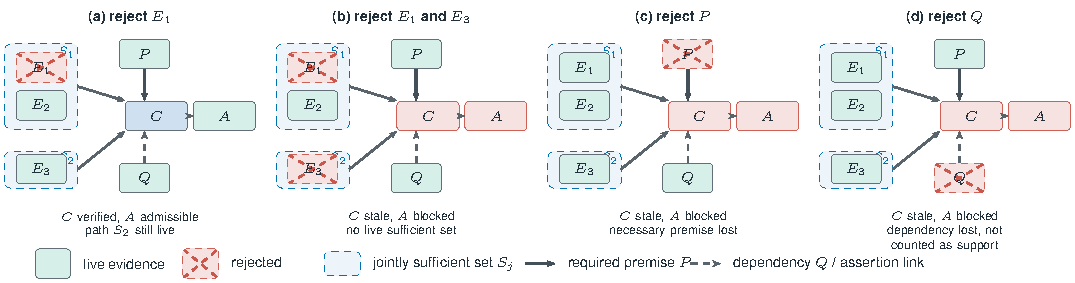
\includegraphics[width=\textwidth]{fig_support.pdf}
\caption{Support-set semantics: one claim $C$ with sufficient sets $S_1=\{E_1,E_2\}$ and $S_2=\{E_3\}$, a necessary premise $P$, a non-epistemic dependency $Q$ and a manuscript assertion $A$, under four revisions. (a) Losing $E_1$ breaks $S_1$ but $S_2$ survives. (b) Losing $E_1$ and $E_3$ leaves no sufficient set. (c) Losing $P$ stales $C$ although both sets are intact. (d) Losing $Q$ stales $C$ without $Q$ ever counting as support. Under binary edges only outcome (a) is reproduced; in (b)--(d) $C$ and $A$ would be left unchanged.}
\label{fig:support}
\end{figure*}

\begin{proposition}\label{prop:conj}
Under singleton-edge semantics $\mathrm{Live}(c)=\bigvee_{e}\mathrm{live}(e)$; for no edge set is this equal to $\mathrm{live}(E_1)\wedge\mathrm{live}(E_2)$ on all assignments.
\end{proposition}
\begin{proof}
If $E_1$ is an edge, the disjunction holds when only $E_1$ is live while the conjunction fails; symmetrically for $E_2$; if neither is an edge the disjunction ignores one of them. \qedhere
\end{proof}
The result is elementary; its point is that support sets are \emph{strictly} more expressive, so losing a conjunction at registration time is a failure distinct from losing an edge.

\paragraph{What the components mean, and what they do not}
By Eqs.~\eqref{eq:live}--\eqref{eq:level}, adding the members of $R(c)$ to every set in $\mathcal{S}(c)$ leaves $\mathrm{Live}$ and $\lambda$ unchanged (only the \texttt{stale}/\texttt{unsupported} label differs for a claim with premises but no sets), so $R(c)$ adds no expressive power. It is a normalization device whose value is registration robustness, since ``common to every alternative'' is declared once and cannot be lost by omitting it from one alternative, and since its failure (a premise flattened into an independent \texttt{supports}) becomes separately measurable. $D(c)$ differs from $R(c)$ only in not entering $\lambda$. Membership itself is a human or agent judgement that TRL takes as input: whether replication is required or reinforcing, whether an assumption or a statistical specification is a premise, a dependency or part of the claim, and whether apparently independent alternatives share a hidden dependence are all outside the model, and evidential support is binary (no partial support, no statistical dependence between sets). A manuscript assertion is a span bound to one or more claims; TRL does not segment text or decide binding granularity, so stale-assertion escape is conditional on that binding. A proposed taxonomy and decision rules for the annotation of these judgements are in \suppl{S7}; agreement on them has not been measured.

\subsection{Invariants and transactions}
\label{sec:txn}
A candidate state is admissible only if it satisfies the following invariants.
\begin{enumerate}
    \item[$I_1$] \textbf{Referential integrity:} every referenced run, evidence, claim, decision or assertion exists.
    \item[$I_2$] \textbf{Reciprocity and derivation:} every relation is recorded on both endpoints, every support-set member is indexed on its claim, and each claim and assertion state equals its derivation.
    \item[$I_3$] \textbf{Supersession and lineage closure:} superseded evidence names an existing replacement; supersession and lineage chains are acyclic.
    \item[$I_4$] \textbf{Decision provenance:} a decision has evidence or a rationale, and a decided or revised decision cites no non-live evidence (including through lineage or run invalidation).
    \item[$I_5$] \textbf{Artifact and verification integrity:} artifact digests match; evidence is not provenance-verified while a recorded tier failed or its run is unfinished.
    \item[$I_6$] \textbf{Manuscript admissibility:} manuscript-referenced claims are supported or verified; every non-outdated assertion is admissible.
    \item[$I_7$] \textbf{Predecessor freshness:} the ledger head still equals the predecessor hash the transaction was built from.
    \item[$I_8$] \textbf{Transition legality:} every object moves only along its state machine (Table~\ref{tab:states}).
\end{enumerate}
$I_1$--$I_6$ and $I_8$ are deterministic checks by ordinary code; $I_7$ is optimistic concurrency control under a local commit lock. An LLM may propose a mutation but cannot override a failed check.

A transaction $\tau=(b,\Delta,a,r)$ carries the exact predecessor hash $b=h(S_t)$, operations $\Delta$, actor $a$ and rationale $r$. It is applied to a private copy, $\widehat S=\mathrm{Apply}(S_t,\Delta)$, and with $H_t$ the head at activation,
\begin{equation}
S_{t+1}=\begin{cases}\widehat S, & H_t=b\ \land\ \bigwedge_{j\in\{1,\dots,6,8\}} I_j(S_t,\widehat S)=1,\\ S_t, & \text{otherwise.}\end{cases}
\label{eq:commit}
\end{equation}
A commit writes a content-addressed snapshot $h_{t+1}=\mathrm{SHA256}(S_{t+1})$ and a hash-chained log record with actor, rationale, operations and before/after hashes. The chain is tamper-\emph{evident} against partial local edits; without an external signature an adversary with full write access could recompute it. Commit-safety (every committed state satisfies the invariants; a stale candidate cannot overwrite a newer head) follows by induction from Eq.~\eqref{eq:commit} and is stated for completeness, not as a deep result.

\begin{proposition}\label{prop:prop}
Let $G$ be the registered graph and $E_0$ the evidence rejected or superseded in one transaction. After commit every claim, assertion and decision has the state that Eqs.~\eqref{eq:live}--\eqref{eq:level} and the state machines assign on $G$ with liveness recomputed on the lineage closure of $E_0$, and nothing outside that closure's dependents changes.
\end{proposition}
\emph{Sketch.} Propagation reconciles exactly the claims linked to a closure member, the assertions bound to them and the decisions citing a member; nothing else is related to a record whose liveness changed. $I_2$ then rejects the commit unless every stored state equals its derivation. \qedhere

The result is sound and complete \emph{with respect to $G$} and silent about the true dependency structure; its content is largely definitional. What is not definitional is the choice of semantics (Proposition~\ref{prop:conj}) and how well $G$ is registered, both tested below. A replacement for superseded evidence does not inherit its support relations; they must be re-established explicitly.

\subsection{Dependency registration}
\label{sec:registration}
Everything above operates on the registered graph, so registration is the principal source of unprotected failure. Writing $G=\mathcal{A}(T)$ for the graph an acquisition process $\mathcal{A}$ (a stage hook, a rule, a person or an LLM) derives from a trajectory $T$, TRL specifies only the revision step applied to $G$; its guarantees (Proposition~\ref{prop:prop}) are conditional on $G$, end-to-end protection cannot exceed the fidelity of $\mathcal{A}$, and we neither implement nor evaluate $\mathcal{A}$ on real trajectories. TRL provides three explicit channels---pipeline hooks called by the stage that knows the semantics, an adapter for ResearchLedger workspaces, and run capture that binds evidence to immutable runs and artifacts---and no automatic edge proposal. Registration provenance is recoverable from the hash-chained log. Against a human-adjudicated gold graph $G^\star$ we define typed precision and recall $\mathrm{P}_{\mathrm{dep}}=|G\cap G^\star|/|G|$ and $\mathrm{R}_{\mathrm{dep}}=|G\cap G^\star|/|G^\star|$ (group and alternative-group edges interchangeable), \emph{object coverage} (gold dependency-bearing objects with every incoming gold edge registered) and \emph{support-set coverage} (gold claims whose full family of sufficient sets and premises is reproduced). Two failures that $\mathrm{R}_{\mathrm{dep}}$ hides are counted separately: a \emph{flattened conjunction} (a group or premise registered as independent \texttt{supports}: no missing edge, wrong semantics) and a \emph{spurious edge} (which can disable protection by creating a fake alternative path).

\section{Implementation and Evaluation Design}
\label{sec:design}
\subsection{Implementation}
TRL is a model-agnostic Python layer (typed dataclasses, JSON, SHA-256, a JSONL log) around AutoResearch's 23-stage workflow; pipeline hooks record evidence, claims, decisions and manuscript bindings, and a fail-closed bridge to ResearchLedger supplies immutable runs, artifact hashing, tracing and manuscript audit (\suppl{S2}). The integrated v2.2 validation build---including support-set revision, transaction recovery, tracked trajectories, paper audit and study tooling---passed 206/206 automated tests across 22 modules in non-overlapping batches; no lint or static-type result is claimed for that run because those executables were unavailable.

\subsection{Evidence hierarchy}
The mechanism benchmarks are generated from mutation classes that correspond closely to TRL's own invariants: excellent conformance tests, weak evidence that the representation captures real revision. We therefore separate developer-run bridge evidence from confirmatory external validation (Table~\ref{tab:hierarchy}).

\begin{table}[t]
\centering
\caption{Evidence hierarchy and current execution status. The tracked-proxy and structural-pilot rows use genuine revision identities but developer-authored bindings; only the top row would provide independent end-to-end construct validation.}
\label{tab:hierarchy}
\scriptsize
\begin{tabularx}{\columnwidth}{>{\raggedright\arraybackslash}p{2.45cm}>{\raggedright\arraybackslash}X>{\raggedright\arraybackslash}p{1.25cm}}
\toprule
Layer & Role & Status \\
\midrule
Confirmatory old/new paper-agent study & real tool outputs, blind dependency/impact truth, matched and native registration & not executed \\
Tracked historical proxy trajectories & immutable runs, supersession, claim/paper invalidation and recovery on genuine revisions & 13/13 executed \\
Authored real-history structural pilot & selective impact semantics on controlled graphs tied to genuine revisions & 10 events executed \\
Human audit study & time-to-locate and stale statements missed & protocol only \\
Mechanism diagnostics & RSM, RSR, HT, DRS, SUP, REG, SM-CONF, TMS-XC, scaling & executed \\
Transaction fault injection & rollback, interrupted recovery, alternative support, concurrent writers & 6/6 executed \\
Integrated software suite & implementation conformance & 206/206 passed \\
\bottomrule
\end{tabularx}
\end{table}

\subsection{Confirmatory old/new paper-agent benchmark (specified, not executed)}
The scientific validation this work needs has ground truth \emph{outside} TRL. The preregistered confirmatory study targets at least 60 genuine semantic revision events from at least 15 repositories (preferred 100--150 events from 25+ repositories). For each event, the old commit is frozen, an executable paper agent is generated where feasible (Paper2Agent provides one concrete standardized substrate \cite{miao2026paper2agent}), a prespecified task is executed, and its outputs and downstream claims are persisted before the historical correction is replayed. Two annotators, blind to registrations and system predictions, independently label affected claims, decisions and assertions and distinguish conjunctive from alternative support; a third adjudicates. Primary outcomes are stale-assertion escape and false invalidation; secondary outcomes include claim precision/recall, selective recomputation, executions avoided relative to full rebuild, recovery correctness, time-to-safe-state, dependency precision/recall and support-set coverage. The preregistered matched-registration systems are: no revision-state management; invalidate-all/full rebuild; downstream reachability; flat binary dependency propagation; AND/OR support-set provenance without transactions; and full TRL. Where feasible, an ATMS or positive-Boolean-provenance implementation is added as a strong formal comparator. Repository, not event, is the resampling unit for 95\% bootstrap intervals. The original EviGraph reconstruction remains a synthetic mechanism comparator only and is not treated as evidence about the native system. Protocols and the human-audit design are in \suppl{S7}; the executed 13-case tracked-proxy study below exercises the downstream ledger lifecycle but not real paper-agent generation or independent annotation.

\begin{figure*}[t]
\centering
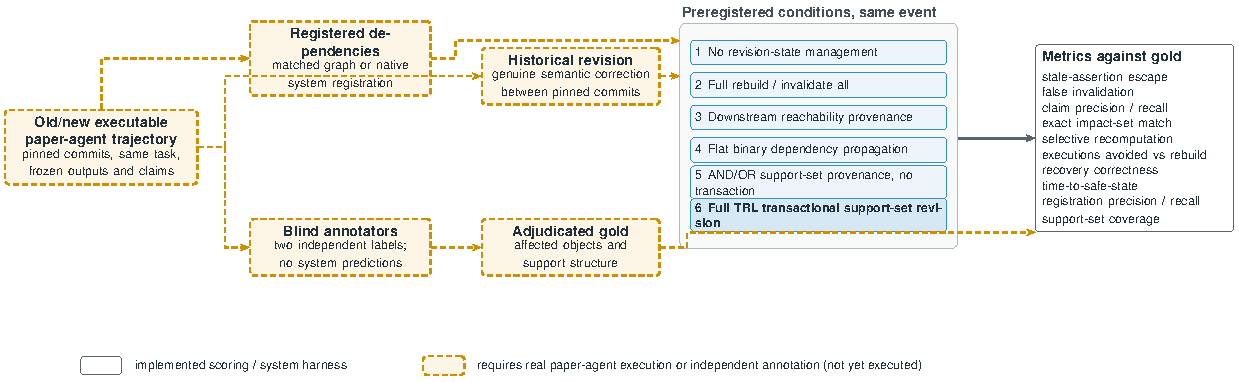
\includegraphics[width=\textwidth]{fig_design.pdf}
\caption{Confirmatory evaluation design. Dashed boxes require real old/new executable-paper-agent trajectories and blind human annotation and have not been executed. The 13-case tracked-proxy bridge study exercises the downstream immutable-run, invalidation, manuscript-audit and recovery path, but does not replace these external acquisition and annotation stages.}
\label{fig:design}
\end{figure*}

\subsection{Mechanism experiments}
\textbf{Conformance.} RSM-1000 (single mutations of a 20-claim state), RSM-SEQ-2500 (25 cumulative mutations $\times$ 100 episodes), RSR-500 (stale-writer races), HT-250 (five classes of local-history corruption), RLV2-400 (seven documented ResearchLedger rule classes) and DRS-1400 (unregistered dependencies) are rerun on the revised core with their original seeds (\suppl{S3}). \textbf{SUP-300 and REG.} A generator builds trajectories with five claim templates (singleton 30\%, conjunctive 25\%, alternative groups 20\%, required premise 15\%, dependency 10\%), lineage, decisions and assertions; three evidence rejections per trajectory yield 815 events with non-empty impact (seed 61). REG corrupts the registered graph by dropped edges, flattened conjunctions or spurious edges (100 trajectories per point, seed 62). The generator authors the gold structure, so these are mechanism diagnostics whose template mix is arbitrary; only direction and mechanism are informative. \textbf{SM-CONF.} An exhaustive check of all 107 ordered state pairs, fuzzing with random legitimate operations, and fuzzing with forbidden direct writes. \textbf{Scaling.} $10^3$--$10^5$ triples at 1, 5 and 20 links per claim, with component timing.

\section{Results}
\label{sec:results}
\subsection{Conformance benchmarks reproduce}
Table~\ref{tab:conf} summarizes the earlier benchmarks. Their result files are identical to the previous prototype's apart from timing fields; claim states now use the typed vocabulary, which changes no count. These results establish that the implementation matches its specification, not that the specification captures real revision. DRS-1400 makes one boundary explicit: when a true dependency is never registered, TRL raises no violation and ledger-reported escape stays at 0\%, while ground-truth escape equals the unregistration rate.

\begin{table}[t]
\centering
\caption{Conformance benchmarks on the revised core (full tables in \suppl{S3}). Residual violations and escape are for the state after all mutations.}
\label{tab:conf}
\scriptsize
\begin{tabularx}{\columnwidth}{l>{\raggedright\arraybackslash}X>{\raggedright\arraybackslash}X}
\toprule
Benchmark & Full TRL & Strongest non-TRL condition \\
\midrule
RSM-1000 & 0 violations, escape 0\%, all legitimate updates committed, all corrupt ones rejected & post-hoc repair: 1.206 violations/trial; raw state: escape 79.9\% \\
RSM-SEQ-2500 & 100/100 episodes consistent & post-hoc repair: 30.0 violations at episode end \\
RSR-500 & OCC + rebase: both updates kept in 500/500 & last-write-wins: lost update in 500/500 \\
HT-250 & 250/250 corruptions detected, 0/25 false positives & --- \\
RLV2-400 & 350/350 corruptions rejected with target rule, 50/50 clean accepted & --- \\
DRS-1400 & ledger escape 0\% at every rate; ground-truth escape $=p_{\text{missing}}$ & --- \\
\bottomrule
\end{tabularx}
\end{table}

\subsection{Support sets and lineage (SUP-300)}
\label{sec:sup_results}
\emph{Synthetic fixtures with generator-authored gold; magnitudes depend on the arbitrary template mix.} With perfect registration, full TRL's set of invalidated claims equalled the oracle's in all 815 events, and it recovered every affected decision and assertion (Fig.~\ref{fig:sup}, Table~\ref{tab:sup}). This is agreement between two implementations of one specification, useful for catching bugs, not evidence about research.

These are representation sanity checks, not comparative evidence: the generator includes templates that singleton edges cannot express, so their failure is by construction. The other conditions fail in ways that map to semantic features. Claim relabelling and TRL without support sets recover 20.5\% of invalidated claims: none of the conjunctive, alternative-group or required-premise claims, and 72.8\% of singleton claims (the rest are lineage taint). A provenance store without transactions \emph{identifies} every affected object but updates none, so all invalid assertions remain admissible (escape 1.00 by state, 0.00 by report). The EviGraph reconstruction recovers every affected claim and assertion but flags 30.3\% of still-justified claims that have an alternative sufficient path, because flagging a whole subgraph cannot tell a lost path from a lost claim; its decision handling depends on whether decisions are graph nodes. Its over-invalidation costs needless regeneration rather than unsound state, and is favored by the given-invalid-node assumption. EG-R is a synthetic reachability baseline: the original system is reported to include further components (for example semantic consistency checks and graph checkpointing) that are not modelled, and no TRL-versus-EviGraph conclusion follows.

\begin{figure*}[t]
\centering
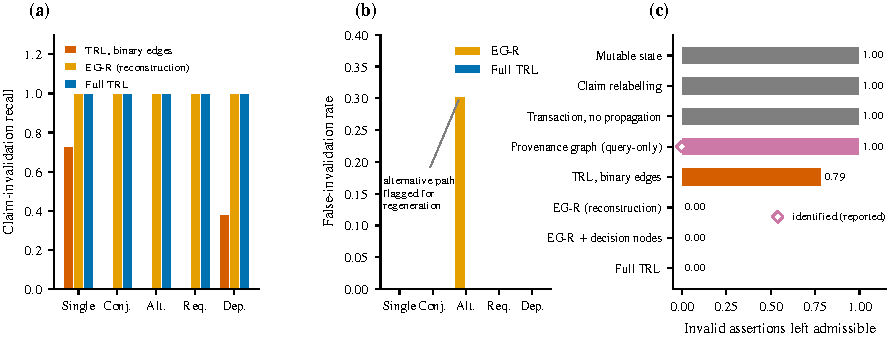
\includegraphics[width=\textwidth]{fig_sup.pdf}
\caption{SUP-300 on synthetic trajectories with perfect registration (815 events). (a) Claim-invalidation recall by claim template: single, conjunctive, alternative-group, required-premise, non-epistemic dependency. (b) False invalidation of still-justified claims: only the reconstruction of EviGraph's mechanism over-invalidates, and only where an alternative sufficient path exists. (c) Invalid assertions left admissible, by condition; the diamond marks what the query-only provenance graph \emph{reports} rather than updates.}
\label{fig:sup}
\end{figure*}

\begin{table}[t]
\centering
\caption{SUP-300 by condition. Recall: invalidated claims recovered; FIR: still-justified claims wrongly invalidated; Escape: invalid assertions left admissible. Values are over stored state unless marked ``reported''.}
\label{tab:sup}
\scriptsize
\begin{tabular}{@{}lcccc@{}}
\toprule
Condition & Recall & FIR & Dec.\ recall & Escape \\
\midrule
Mutable state & 0.000 & 0.000 & 0.000 & 1.000 \\
Claim relabelling & 0.205 & 0.000 & 0.000 & 1.000 \\
Provenance graph, updated & 0.000 & 0.000 & 0.000 & 1.000 \\
Provenance graph, reported & 1.000 & 0.070 & 1.000 & 0.000 \\
Transaction, no propagation & 0.000 & 0.000 & 0.000 & 1.000 \\
EG-R (reconstruction) & 1.000 & 0.070 & 0.000 & 0.000 \\
TRL, binary edges & 0.205 & 0.000 & 0.757 & 0.787 \\
\textbf{Full TRL} & \textbf{1.000} & \textbf{0.000} & \textbf{1.000} & \textbf{0.000} \\
\bottomrule
\end{tabular}
\end{table}

\subsection{Registration sensitivity (REG)}
\label{sec:reg_results}
Fig.~\ref{fig:reg} shows escape of full TRL as the registered graph is corrupted; all observations are on synthetic fixtures. \emph{Escape rises much faster than edge recall falls}: dropping 5\% of true edges gives $\mathrm{R}_{\mathrm{dep}}=0.947$ and support-set coverage 0.890, yet 17.2\% of invalidated assertions escape; at 10\% dropped, recall is 0.902 and escape 24.2\%. Losing one member of a conjunction removes the whole claim from protection, and one lost lineage edge can do the same downstream. Over the seven drop rates escape $=0.074+1.52\,(1-\mathrm{R}_{\mathrm{dep}})$ ($R^2=0.977$, aggregate points, $n=7$; a description of these fixtures, not a law), which is why edge recall alone is an insufficient registration metric. \emph{Flattening} produces no missing edge yet yields 57.1\% escape when every conjunction is flattened. \emph{Spurious} edges with perfect recall still raise escape (23.4\% at 10\%, 61.2\% at 30\%): an extra \texttt{supports} edge creates a fake alternative path that keeps an invalid claim alive, so registration precision matters for protection, not only recall. TRL without support sets fails at every point.

\begin{figure*}[t]
\centering
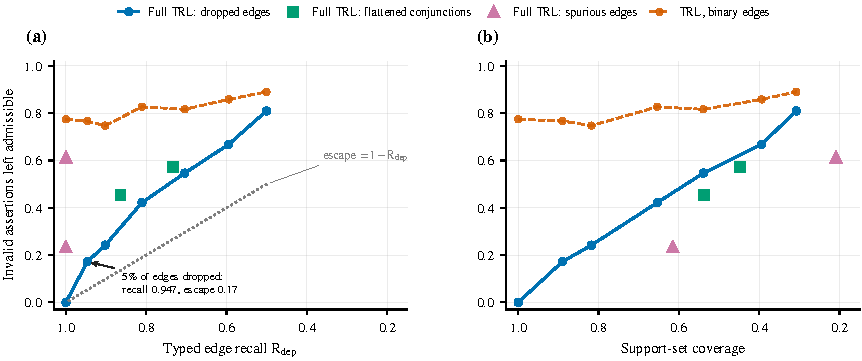
\includegraphics[width=\textwidth]{fig_reg.pdf}
\caption{Protection under registration corruption (100 synthetic trajectories per point). Escape is the fraction of invalid manuscript assertions left admissible. (a) Against typed edge recall; the dotted line is escape $=1-\mathrm{R}_{\mathrm{dep}}$. (b) Against support-set coverage. Dropped edges, flattened conjunctions and spurious edges are separate corruption processes; the dashed line is TRL restricted to binary edges.}
\label{fig:reg}
\end{figure*}

\subsection{State-machine conformance (SM-CONF)}
The exhaustive matrix agreed with the documented relations on all 107 ordered pairs. In 150 fuzzing episodes (seed 53), 4,582 of 4,611 operations committed with no invariant violation, \emph{none} of the legitimate operations was rejected as an illegal transition, and the 29 rejections were all the intended \texttt{stale\_decision}. The fuzzer exercised 44 of 48 table edges; all 500 forbidden direct writes and 100 direct writes contradicting the derivation were rejected. The informative outcome is what the first pass did to the design: our initial claim machine declared \texttt{stale} sticky and forbade \texttt{supported}$\to$\texttt{unsupported}, but re-supporting a stale claim with unaccepted evidence and declaring an unaccepted required premise reach exactly those transitions. We corrected the specification: claim states are derived and the operative constraint is agreement with the derivation. SM-CONF tests consistency of the implementation with its own tables, not that they are the right tables for any workflow.

\subsection{Truth-maintenance cross-check (TMS-XC)}
\label{sec:tms_xc}
On 300 synthetic trajectories (seed 61; 900 events per graph) we recomputed each revision's affected objects with the oracle, a Doyle-style JTMS, a de Kleer-style ATMS and full TRL, on the gold graph and on graphs with dropped, flattened or spurious edges. JTMS and ATMS matched the oracle on all 3,600 events; TRL matched on 3,551. Its 49 divergences all have mechanical causes (\suppl{S8}): 25 are assertions already blocked by an unsupported claim, which undergo no state transition, and 24 are mistyped duplicate edges on one (evidence, claim) pair, which collide in TRL's one-relation-per-pair model and make it over-invalidate. This is agreement among implementations of one semantics, not evidence about real research; a relation model with several relations per pair would remove the collision.

\subsection{Scaling}
\label{sec:scale_results}
Fig.~\ref{fig:scale} shows one revision on a committed archive of $10^4$ to $10^5$ triples (three records each). Timings are from a noisy 24-thread Windows laptop (the earlier prototype's code is $\approx\!3.5\times$ slower here than its published numbers, and medians at $10^3$ triples varied by up to $3\times$), so only scales $\ge10^4$ are interpreted. Three findings are robust. \emph{Propagation is not the bottleneck}: 5--30 ms through $5\times10^4$ triples and 0.2 s at $10^5$, under 1\% of a revision. \emph{Everything else is linear in archive size, and the full-snapshot design is the bottleneck}: a revision takes about 2 s at $10^4$ triples, 9--18 s at $5\times10^4$ and 65 s at $10^5$, with a 72 MB snapshot rewritten per commit. \emph{Storage flushing is not the cost at scale}: with \texttt{fsync} disabled, commit time at $\ge5\times10^4$ triples is unchanged. A single-pass store (one serialization, no deep copy) keeps hashes identical, roughly halves revision time and cuts snapshots by 37\%, but changes constants, not asymptotics. Density matters less than record count (at $10^4$ triples, 1 to 20 links per claim raises a revision from 2.0 to 2.5 s). We did not run $5\times10^5$ triples; supporting that regime needs a persistent Merkle or delta structure with lazy loading and incremental validation, which we describe but do not implement. Full tables are in \suppl{S6}.

\begin{figure*}[t]
\centering
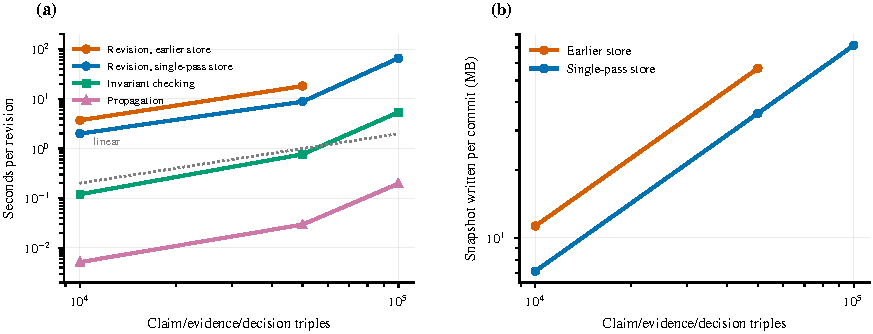
\includegraphics[width=\textwidth]{fig_scale.pdf}
\caption{Scaling of a single evidence-rejection revision, $10^4$--$10^5$ triples (median of 3--5). (a) Time per revision, invariant checking and propagation under the earlier and the single-pass store; the dotted line has unit log-log slope. (b) Snapshot size, which is also the number of bytes written per commit.}
\label{fig:scale}
\end{figure*}

\subsection{Historical revisions, tracked proxy trajectories and fault injection (development evidence)}
\label{sec:hist_replay_main}
The source audit identified 13 genuine semantic revisions across nine scientific-software repositories (\texttt{POP-TOOLS}, \texttt{scanpy}, \texttt{squidpy}, \texttt{TabPFN}, \texttt{SAELens}, \texttt{Compass}, \texttt{scvi-tools}, \texttt{seurat}, \texttt{scikit-learn}). Replaying the smallest changed semantic unit reproduced the documented old/new behavioral, numerical, data or configuration difference in 13/13 cases (\suppl{S9}). The cases include sparse normalization, a statistical-variance correction, calibration under majority downsampling, feature subsampling, sequence-boundary handling, PCA setup, duplicated data removal and scientific defaults. These are narrow semantic replays rather than full historical repository builds.

We then passed every case through a deterministic paper-agent proxy as two separate immutable ResearchLedger runs. The old output was frozen as provenance-verified evidence for a claim; the historical revision superseded that evidence transactionally; and the revised output was attached as replacement evidence and verified. All 13 trajectories produced different old/new artifact hashes and completed the same expected lifecycle (Table~\ref{tab:tracked_proxy}): the claim was \texttt{supported} before revision, became \texttt{hypothesis} after the old evidence was superseded, and returned to \texttt{supported} after replacement verification. An explicit manuscript provenance marker naming the superseded evidence was flagged stale in 13/13 cases and recovered in 13/13 after the marker was changed to the replacement evidence. Every final workspace had zero validation errors. Median local transaction-only time to the safe invalidated state was 9.6 ms and median recovery bookkeeping after the revised output already existed was 15.0 ms; old/new proxy tool runs were about 2.9--3.0 s and were dominated by local process/environment capture. These timings are implementation diagnostics, not Paper2Agent or production benchmarks.

\begin{table}[t]
\centering
\caption{Ledger-integrated tracked proxy trajectories over 13 genuine historical revisions. Bindings and proxy tools were developer-authored; this is bridge/conformance evidence, not independent external validation.}
\label{tab:tracked_proxy}
\scriptsize
\begin{tabularx}{\columnwidth}{>{\raggedright\arraybackslash}Xr}
\toprule
Outcome & Result \\
\midrule
Historical revisions / repositories & 13 / 9 \\
Documented old/new semantic change reproduced & 13/13 \\
Old/new artifact hash changed & 13/13 \\
Claim \texttt{supported}$\to$\texttt{hypothesis} after supersession & 13/13 \\
Explicit superseded-evidence manuscript marker flagged stale & 13/13 \\
Replacement evidence restored \texttt{supported} claim & 13/13 \\
Recovered manuscript marker no longer stale & 13/13 \\
Final workspace validation errors & 0 in 13/13 \\
Median time to safe invalidated state$^\dagger$ & 9.6 ms \\
Median recovery bookkeeping$^\dagger$ & 15.0 ms \\
\bottomrule
\multicolumn{2}{l}{\scriptsize $^\dagger$Excludes generation of the revised tool output; local proxy diagnostic only.}
\end{tabularx}
\end{table}

We separately fault-injected the multi-file revision transaction under six deterministic checks. All passed, including forced write failure and simulated mid-transaction crash with exact pre-image restoration, 11/11 tested entity-write fault positions on an 11-file revision, preservation of a claim when one of two alternative sufficient support paths remained live, and two independent concurrent revision processes both reaching the expected final state. On a separate authored 10-event structural pilot, support-set provenance without transactions and full TRL both reached 10/10 exact impact identification; flat binary edges reached 6/10; unconditional downstream reachability and invalidate-all/full rebuild reached 4/10 exact matches because they over-invalidated claims retaining an alternative sufficient support path. A repository-clustered bootstrap over eight repository clusters gave a median TRL-minus-binary-edge claim-recall difference of 0.40 (95\% percentile interval $[0.111,0.700]$) and a median TRL-minus-support-set-provenance exact-match difference of 0.0 ($[0,0]$). Because the impact graphs and gold sets were authored for mechanism development, these intervals are descriptive sensitivity analyses, not external-validation uncertainty. The decomposition is important: AND/OR support semantics explain selective impact identification on this pilot; the transaction layer contributes atomic multi-file state change, rollback, crash recovery, freshness/serialization and auditable history. The integrated validation package passed 206/206 automated tests across 22 modules.

\section{Discussion and Limitations}
\label{sec:discussion}
\subsection{Implications}
The results suggest two separable layers of reliability in research agents: \emph{artifact reliability} (code runs, citations resolve, numbers match stored results) and \emph{revision integrity} (when an artifact changes, the system knows what is no longer justified). Executable-paper systems such as Paper2Agent make the distinction operational: a tool may remain executable while a historical semantic correction changes the output on which persisted claims depend. The tracked-proxy study shows that the implemented ledger can carry such an old/new change through immutable runs, stale-evidence detection and recovery, although it does not establish that a native paper agent will register the right dependencies. The diagnostics add two lessons for anyone building the second layer. First, protection depends on registration quality in ways that edge recall understates: a lost conjunction member, a flattened premise or a single spurious alternative path each disables protection for a whole claim, so registration should be reported as precision, recall and support-set coverage together. Second, a system that can \emph{list} affected objects but does not reconcile stored state leaves invalid assertions admissible; whether identification suffices in practice is a design question that must be measured on real trajectories rather than assumed. Our design principle, from this implementation and not established in general, is that global integrity conditions should be deterministic checks, since such a check cannot be argued out of failing by the process whose output it gates.

\subsection{Threats to validity and limitations}
\begin{itemize}
    \item \textbf{Construct and external validity: no independent real-paper-agent result.} Synthetic experiments still use generator-authored gold. The 13 historical revision identities and changed semantics are genuine, and the tracked proxy executes the full ledger invalidation/recovery lifecycle, but the executable is a deterministic paper-agent proxy rather than a Paper2Agent-generated MCP and the claim/evidence bindings are developer-authored rather than blind human labels. Thus the study does not establish how often real agents register the right dependencies, how native agent outputs change across revisions, or how well TRL agrees with independent scientific judgement; these remain the confirmatory study's purpose.
    \item \textbf{Comparator validity.} EG-R is a reconstruction of published mechanism under assumptions that favor it; no original system was run, and no human used the system. Conclusions about EviGraph itself are out of scope.
    \item \textbf{Semantic warrant.} A support set is a declaration checked for structure, and provenance-verified does not mean well designed or validly inferred. The schema has no graded contradiction, no claim-to-claim or decision-to-claim dependency, no evidence-quality model, and no notion of statistical dependence between apparently independent evidence.
    \item \textbf{Auditability.} No person has used TRL. We claim only deterministic checking of invariants, digests and the export gate and tamper evidence against local edits; we do not claim that reviewers find stale evidence faster or miss fewer stale statements (\suppl{S7} is a protocol only).
    \item \textbf{Registration.} Real registration quality is not measured, and automatic edge proposal from manuscript text or run logs is not implemented.
    \item \textbf{Internal and statistical validity.} Diagnostics use fixed seeds and one generator configuration. The 10-event historical structural pilot is authored development evidence; its repository-clustered interval quantifies sensitivity within that pilot, not population-level uncertainty. Timing is from one local machine, and the millisecond tracked-proxy transaction times exclude external agent generation and revised computation.
    \item \textbf{Scale.} Measured to $10^5$ triples on full snapshots; beyond that requires a persistent Merkle or delta store with lazy loading.
    \item \textbf{Novelty.} Truth maintenance, provenance, argumentation and predecessor-anchored activation already exist \cite{doyle1979tms,buneman2001provenance,dung1995acceptability,he2026continuity}; the support-set model is a restricted, declared fragment, not an advance on them. Any novelty is in the composition (typed research objects, transactional commit, manuscript gating, registration metrics), and the literature survey behind it is narrow.
\end{itemize}
Because a provenance layer lowers the cost of tracing but not the cost of judging, it should support, not replace, human review of generated manuscripts (\suppl{S9}).

\section{Conclusion}
We presented a transactional research-state layer whose revision semantics rest on declared support sets, evidence lineage and typed state machines, and whose strongest evidence state is provenance-verified rather than scientifically valid. Synthetic conformance experiments show that the implementation matches its specification and that selective invalidation requires AND/OR support semantics rather than flat singleton edges. Registration diagnostics show that missing, flattened and spurious dependencies can each defeat protection. Beyond synthetic fixtures, 13 genuine historical software revisions from nine repositories reproduced their documented semantic change, and all 13 completed an immutable-run proxy lifecycle in which superseding old evidence moved a supported claim to hypothesis, explicit stale manuscript provenance was detected, and verified replacement evidence restored the claim; local fault injection separately exercised rollback and crash recovery. These bridge results materially strengthen implementation confidence but do not close the central external-validity gap. We therefore do not claim that real paper agents remain scientifically valid under revision. The decisive next study is preregistered: old/new executable-paper-agent replay on at least 60 genuine revision events from at least 15 repositories, with two blind annotators, adjudication, strong logical baselines and repository-clustered uncertainty.

\section*{Data and Code Availability}
Code, seeds, result files, the 13-case tracked-trajectory runner, transaction fault-injection outputs, blind annotation packets and aggregation/adjudication tooling, confirmatory preregistration, and protocols are in the accompanying v2.2 validation package (\suppl{S10}); the package is frozen by SHA-256.

\printbibliography

\end{document}
